\section{Arquitetura}

Nesta seção, proporciona-se uma visão abrangente da arquitetura da aplicação, englobando os padrões e princípios de design adotados na concepção da solução. Além disso, são detalhadas as tecnologias, \textit{\gls{Frameworks}} e bibliotecas utilizados no desenvolvimento da aplicação, acompanhados das considerações referentes à segurança e escalabilidade incorporadas na arquitetura da solução.

\subsection{Desenho da aplicação}

Para o projeto em questão, adotou-se uma abordagem convencional de arquitetura web cliente-servidor, em que a interface \textit{\gls{Front-end}} se interconecta com a \ac{api} \textit{\gls{Back-end}} por meio dos protocolos HTTP disponíveis. É crucial ressaltar que uma \ac{api} externa fornecida pela \textit{\gls{Rawg}} foi empregada, ampliando significativamente a disponibilidade de informações acerca de jogos, como datas de lançamento, avaliações, plataformas e outros dados relevantes. Além disso, foi utilizada a \ac{api} do \gls{MercadoPago} para auxiliar no processamento de transações monetárias para as assinaturas premium. A Figura \ref{DesenhoArquitetura} oferece uma representação completa do diagrama arquitetural implementado no sistema.

\begin{figure}[H]
    \centering
	\caption{Desenho da Arquitetura}
    \label{DesenhoArquitetura}
    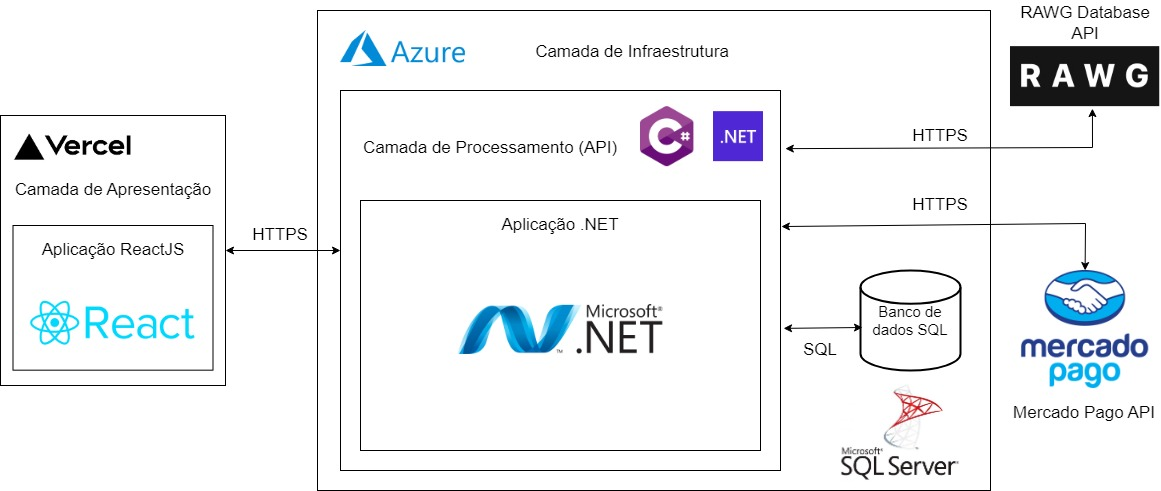
\includegraphics[scale = 0.37]{imagens/arquitetura/desenho_arquitetura.jpg}	
    \fonte{Os Autores}
\end{figure}

% Tecnologias e Ferramentas
\subsection{Tecnologias}

Nesta seção, apresentar-se-á uma visão geral de todas as tecnologias escolhidas para a implementação da aplicação, incluindo as linguagens de programação, \textit{\gls{Framework}} e bibliotecas utilizadas.

\subsubsection{Back-end}

No âmbito do \textit{\gls{Back-end}}, a escolha recaiu sobre a linguagem de programação \textit{\gls{Csharp}}, em concomitância com a plataforma de desenvolvimento e o \textit{Framework} \textit{\gls{.NET}}. Por conseguinte, foi concebida uma \ac{api} voltada ao gerenciamento da aplicação e à manipulação dos dados. No tocante à criação das tabelas do banco de dados e à gestão dos dados existentes, recorreu-se ao pacote \textit{\gls{Entity}}, que desempenha a função de \ac{orm} no âmbito deste projeto.

\subsubsection{Front-end}

No contexto do desenvolvimento do \textit{\gls{Front-end}} da aplicação, a linguagem de programação \textit{\gls{Javascript}} foi selecionada, em conjunto com a biblioteca \textit{\gls{React}}, para a construção dos componentes essenciais da plataforma. Adicionalmente, o \ac{css} foi empregado para conferir estilo às páginas, visando aprimorar a atratividade visual das interfaces aos olhos dos usuários. Por último, foram incorporadas bibliotecas destinadas a animação e ao controle de formulários, com o propósito de proporcionar suporte e otimizar a condução do processo de desenvolvimento da aplicação.

\subsubsection{Banco de dados}

Para a gestão e acesso aos dados, a opção recaiu sobre o \textit{\gls{Sqlserver}}, utilizando uma instância fornecida pelo serviço Azure. No processo de estruturação das tabelas e aplicação das etapas de normalização, a escolha foi direcionada à utilização do pacote \textit{\gls{Entity}}, desenvolvido pela \textit{\gls{Microsoft}}.

\subsubsection{Infraestrutura}

Quanto ao processo de \textit{\gls{Deploy}} da aplicação, é importante ressaltar que o \textit{\gls{Front-end}} foi devidamente hospedado na plataforma \textit{\gls{Vercel}}, enquanto o \textit{\gls{Back-end}} na plataforma da \textit{\gls{Azure}}.

\subsubsection{Escalabilidade}

As ferramentas disponibilizadas pela plataforma \textit{\gls{Azure}} foram empregadas no decorrer deste projeto, notadamente o sistema de dimensionamento automático. Tal emprego teve por objetivo primordial a adequação dinâmica da aplicação, alinhando-a de maneira precisa às demandas e necessidades apresentadas.

\subsubsection{APIs Externas}
Foram utilizadas duas \ac{api} externas para fornecer recursos e ferramentas à aplicação, sendo uma pertencente à \textit{\gls{Rawg}} e a outra, ao \gls{MercadoPago}.

A \ac{api} da \textit{\gls{Rawg}} foi utilizada por fornecer um
vasto conjunto de informações pertinentes ao universo dos jogos digitais, abrangendo
aspectos como o ano de lançamento, o estúdio desenvolvedor, os criadores e outros detalhes
relevantes.

Já a \ac{api} do \gls{MercadoPago} foi empregada para fornecer apoio ao fluxo de pagamento do plano premium fornecido pela aplicação, já que ela traz consigo todos os recursos necessários para realizar essas transações de forma segura.